\apendice{Documentación técnica de programación}

\section{Introducción}

Este anexo recoge la documentación técnica de programación de \textit{UBU E-R App}. Su objetivo es servir como guía práctica para futuros desarrolladores que deban instalar el proyecto, ejecutarlo en local, comprender su estructura interna y continuar su evolución de forma controlada.

A diferencia del Anexo C, centrado en la especificación de diseño de la aplicación, este anexo tiene un enfoque operativo. Por ello, no se repiten en detalle los diagramas de arquitectura, el metamodelo del diagrama ni el proceso completo de transformación relacional. En su lugar, se describen los aspectos necesarios para trabajar con el código fuente: organización del repositorio, dependencias principales, scripts disponibles, ejecución local, construcción de la aplicación y pruebas.

El proyecto corresponde a la evolución de una aplicación web heredada para la edición de diagramas Entidad--Relación. La aplicación está desarrollada con React y utiliza mxGraph como librería principal para la representación y manipulación del lienzo visual. Durante el desarrollo del TFG se ha mantenido un criterio conservador: estabilizar y ampliar la herramienta sin reescribirla desde cero, preservando la coherencia entre el lienzo gráfico, la representación interna del diagrama, la validación, la transformación al modelo relacional, la generación de SQL y los mecanismos de persistencia.

\section{Estructura de directorios}

El repositorio del proyecto se organiza de forma convencional para una aplicación web basada en React. En la raíz del proyecto se encuentran los ficheros de configuración, la definición de dependencias, los scripts de ejecución y las carpetas principales de código, pruebas, documentación y recursos.

La estructura general más relevante es la siguiente:

\begin{verbatim}
/
+-- assets/
+-- docs/
+-- public/
+-- scripts/
+-- src/
+-- tests/
+-- package.json
+-- package-lock.json
+-- README.md
+-- LICENSE
+-- biome.json
+-- playwright.config.js
\end{verbatim}

A continuación se describe la finalidad de los directorios y ficheros principales:

\begin{itemize}
\item \texttt{assets/}: contiene recursos gráficos generales del proyecto, como imágenes o animaciones utilizadas en la documentación del repositorio.

\item \texttt{docs/}: contiene documentación auxiliar del proyecto. Dentro de esta carpeta se incluyen materiales de análisis, documentación \LaTeX{} y recursos empleados en la memoria y anexos.

\item \texttt{public/}: contiene los recursos estáticos servidos directamente por la aplicación React.

\item \texttt{scripts/}: contiene scripts auxiliares de automatización. En particular, se utiliza para generar información de versión o construcción antes de arrancar o compilar la aplicación.

\item \texttt{src/}: contiene el código fuente principal de la aplicación. Es la carpeta más relevante desde el punto de vista del desarrollo funcional del editor.

\item \texttt{tests/}: contiene las pruebas automatizadas del proyecto, tanto pruebas unitarias como pruebas de extremo a extremo.

\item \texttt{package.json}: define las dependencias del proyecto, sus metadatos y los scripts disponibles para instalación, ejecución, pruebas, análisis y construcción.

\item \texttt{package-lock.json}: fija las versiones concretas de las dependencias instaladas, permitiendo reproducir el entorno de forma más estable.

\item \texttt{README.md}: proporciona una descripción general del proyecto, sus funcionalidades principales, tecnología utilizada, instalación básica, pruebas y licencia.

\item \texttt{LICENSE}: contiene la licencia del proyecto. La versión actual se distribuye bajo licencia MIT.

\item \texttt{biome.json}: contiene la configuración de Biome, herramienta empleada para tareas de formato y análisis estático del código.

\item \texttt{playwright.config.js}: contiene la configuración de Playwright para las pruebas de extremo a extremo.

\end{itemize}

La carpeta \texttt{src/} concentra la implementación de la aplicación. Su estructura actual separa el editor visual, las reglas del dominio E/R, la transformación relacional, la generación SQL y la internacionalización:

\begin{verbatim}
src/
+-- components/
| +-- DiagramEditor/
+-- domain/
| +-- er/
| +-- relational/
+-- i18n/
+-- services/
+-- App.js
+-- buildInfo.js
+-- index.js
+-- styles.css
\end{verbatim}

Los elementos principales de esta carpeta son:

\begin{itemize}
\item \texttt{index.js}: punto de entrada de la aplicación React.

\item \texttt{App.js}: componente superior de la aplicación.

\item \texttt{buildInfo.js}: fichero con información de construcción utilizada por la aplicación.

\item \texttt{styles.css}: estilos globales compartidos por la interfaz.

\item \texttt{components/DiagramEditor/}: contiene el editor visual de diagramas Entidad--Relación. Incluye el componente principal, hooks específicos, paneles de interfaz, estilos y utilidades de integración con mxGraph.

\item \texttt{domain/er/}: contiene reglas y funciones auxiliares propias del dominio Entidad--Relación, como gestión de entidades, relaciones, atributos, jerarquías ISA, normalización y validación.

\item \texttt{domain/relational/}: contiene la lógica de transformación desde la representación E/R hacia una representación relacional intermedia.

\item \texttt{services/}: contiene servicios de generación y renderizado de SQL.

\item \texttt{i18n/}: contiene el contexto de idioma y las cadenas de traducción utilizadas por la interfaz.

\end{itemize}

Dentro del editor principal, la estructura se ha reorganizado para reducir la concentración de responsabilidades en un único fichero:

\begin{verbatim}
src/components/DiagramEditor/
+-- DiagramEditor.js
+-- hooks/
+-- panels/
+-- styles/
+-- utils/
\end{verbatim}

El fichero \texttt{DiagramEditor.js} actúa como componente orquestador del editor. Mantiene las referencias principales del lienzo, coordina la inicialización de mxGraph, compone los hooks y paneles, y conecta la interacción visual con la representación interna del diagrama.

La carpeta \texttt{hooks/} agrupa lógica de acciones y servicios asociados al editor:

\begin{verbatim}
hooks/
+-- useAttributeActions.js
+-- useDeletionActions.js
+-- useDiagramHistory.js
+-- useDiagramPersistence.js
+-- useIsaActions.js
+-- useRelationActions.js
\end{verbatim}

Estos hooks encapsulan responsabilidades como la gestión del historial, la persistencia, las acciones sobre atributos, relaciones, jerarquías ISA y operaciones de borrado.

La carpeta \texttt{panels/} contiene componentes de interfaz del panel lateral:

\begin{verbatim}
panels/
+-- DiagramEditorGlobalActions.js
+-- DiagramEditorPanelControls.js
+-- DiagramEditorSidebar.js
\end{verbatim}

En ella se separan las acciones generales del editor, los controles compartidos y las acciones contextuales dependientes de la selección actual.

Por último, la carpeta \texttt{utils/} contiene utilidades agrupadas por responsabilidad técnica:

\begin{verbatim}
utils/
+-- graph/
+-- mxStyles/
+-- persistence/
+-- rendering/
+-- selection/
+-- sync/
+-- toolbar/
+-- validation/
\end{verbatim}

Estas utilidades incluyen la integración con mxGraph, los estilos visuales de las celdas, la importación y exportación de diagramas, el renderizado de elementos, la selección, la sincronización entre modelo y grafo, la barra de herramientas y los mensajes de validación mostrados al usuario.

Esta organización busca facilitar el mantenimiento del proyecto sin ocultar el carácter heredado de la aplicación. Algunas partes, especialmente la inicialización de mxGraph y determinados efectos ligados al ciclo de vida del editor, permanecen en el componente principal por prudencia, ya que están fuertemente acopladas al funcionamiento del lienzo visual.

\section{Manual del programador}

Esta sección describe los pasos necesarios para preparar el entorno de desarrollo, instalar las dependencias, ejecutar la aplicación en local y utilizar los scripts principales del proyecto. El objetivo no es documentar cada fichero de la aplicación, sino proporcionar una guía suficiente para que otro desarrollador pueda continuar el trabajo sin depender únicamente del conocimiento previo del autor.

\subsection{Requisitos previos}

Para trabajar con el proyecto es necesario disponer de un entorno de desarrollo web basado en Node.js y npm. La aplicación se ejecuta completamente en el navegador y no requiere la instalación de un servidor de bases de datos ni de un backend propio.

Los requisitos principales son:

\begin{itemize}
\item \textbf{Node.js}: entorno de ejecución necesario para instalar dependencias, arrancar la aplicación y generar la versión de producción.

\item \textbf{npm}: gestor de paquetes utilizado para instalar las dependencias declaradas en el fichero \texttt{package.json} y ejecutar los scripts del proyecto.

\item \textbf{Navegador web moderno}: necesario para utilizar la aplicación durante el desarrollo. Se recomienda emplear un navegador actualizado, especialmente al ejecutar pruebas manuales sobre el lienzo.

\item \textbf{Editor de código}: se puede utilizar cualquier editor compatible con proyectos JavaScript. Durante el desarrollo se ha trabajado principalmente con Visual Studio Code.

\end{itemize}

El proyecto incluye un fichero \texttt{.node-version}, que sirve como referencia de la versión de Node.js utilizada en el entorno de desarrollo. Es recomendable respetar dicha versión o, al menos, emplear una versión compatible con \texttt{react-scripts} y con las dependencias instaladas.

\subsection{Instalación de dependencias}

Una vez descargado o clonado el repositorio, la instalación de dependencias se realiza desde la raíz del proyecto mediante el siguiente comando:

\begin{verbatim}
npm install
\end{verbatim}

Este comando lee el fichero \texttt{package.json} y utiliza \texttt{package-lock.json} para instalar versiones concretas de las dependencias. Es importante conservar el fichero \texttt{package-lock.json}, ya que ayuda a reproducir el entorno de instalación y reduce diferencias entre equipos.

Las dependencias principales de ejecución incluyen React, mxGraph, Material UI, fuentes de Roboto, utilidades de notificación y librerías auxiliares de interfaz. Las dependencias de desarrollo incluyen herramientas de pruebas, cobertura, análisis estático y automatización.

\subsection{Ejecución en entorno de desarrollo}

Para arrancar la aplicación en local se utiliza el script:

\begin{verbatim}
npm start
\end{verbatim}

Antes de ejecutar el servidor de desarrollo, el proyecto lanza automáticamente el script \texttt{prestart}, encargado de generar información de construcción mediante \texttt{scripts/generateBuildInfo.js}. Después, \texttt{react-scripts} inicia la aplicación en modo desarrollo.

Una vez arrancada, la aplicación queda disponible en el navegador en la dirección local indicada por la terminal, normalmente:

\begin{verbatim}
http://localhost:3000
\end{verbatim}

Durante esta ejecución se pueden realizar pruebas manuales del editor: creación de entidades, relaciones, atributos, jerarquías ISA, validación del diagrama, generación de SQL, importación y exportación de diagramas y comprobación de la persistencia local.

\subsection{Construcción de la aplicación}

Para generar una versión de producción se utiliza el comando:

\begin{verbatim}
npm run build
\end{verbatim}

De forma análoga al arranque en desarrollo, antes de construir la aplicación se ejecuta el script \texttt{prebuild}, que actualiza la información de construcción. Posteriormente, \texttt{react-scripts} genera una versión optimizada de la aplicación en la carpeta \texttt{build/}.

La carpeta \texttt{build/} contiene los ficheros estáticos resultantes, preparados para ser servidos por una plataforma de despliegue web. En el proyecto actual, el despliegue se realiza sobre Vercel, que se encarga de construir y publicar la aplicación a partir del repositorio.

La aplicación no depende de un backend propio. La lógica principal se ejecuta en el navegador del usuario y la persistencia ordinaria del diagrama se realiza mediante \texttt{localStorage} y mediante ficheros JSON importados o exportados por el usuario.

\subsection{Scripts disponibles}

Los scripts principales del proyecto están definidos en el fichero \texttt{package.json}. Los más relevantes para un desarrollador son los siguientes:

\begin{itemize}
\item \texttt{npm start}: arranca la aplicación en modo desarrollo.

\item \texttt{npm run build}: genera la versión de producción de la aplicación.

\item \texttt{npm test}: ejecuta la batería de pruebas unitarias con Vitest, excluyendo las pruebas de extremo a extremo.

\item \texttt{npm test -- --run}: ejecuta las pruebas unitarias en modo no interactivo, adecuado para una comprobación puntual antes de cerrar cambios.

\item \texttt{npm run test:e2e}: ejecuta las pruebas de extremo a extremo con Playwright.

\item \texttt{npm run test:coverage}: ejecuta las pruebas unitarias y genera información de cobertura.

\item \texttt{npm run lint}: ejecuta Biome sobre la carpeta \texttt{src/} para detectar y corregir problemas de análisis estático cuando sea posible.

\item \texttt{npm run format}: aplica el formateo de Biome sobre la carpeta \texttt{src/}.

\end{itemize}

En el trabajo diario se recomienda ejecutar, como mínimo, las pruebas unitarias y el análisis estático antes de considerar cerrado un cambio. Para modificaciones que afecten al comportamiento visual del editor, a la interacción con mxGraph, a la persistencia o a flujos completos de usuario, también conviene ejecutar las pruebas de extremo a extremo o realizar una revisión manual específica en el navegador.

\subsection{Consideraciones sobre el entorno}

El proyecto procede de una base heredada y utiliza \texttt{react-scripts}, por lo que pueden aparecer advertencias asociadas a dependencias internas o herramientas de construcción. Durante la revisión final del código se comprobó que dichas advertencias no bloqueaban la ejecución, las pruebas ni la generación de la build.

Si aparecen errores al instalar o ejecutar el proyecto, se recomienda revisar primero:

\begin{itemize}
\item la versión de Node.js utilizada;
\item que las dependencias se hayan instalado desde la raíz del proyecto;
\item que no existan restos inconsistentes en \texttt{node\_modules/};
\item que se esté usando el fichero \texttt{package-lock.json} incluido en el repositorio;
\item que Playwright tenga instalados los navegadores necesarios si se van a ejecutar pruebas de extremo a extremo.
\end{itemize}

En caso de problemas persistentes de dependencias, una estrategia habitual consiste en eliminar la carpeta de dependencias instaladas y reinstalar el proyecto mediante \texttt{npm install}. Esta operación debe realizarse con prudencia, evitando modificar manualmente el fichero \texttt{package-lock.json} salvo que se esté actualizando una dependencia de forma justificada.

\section{Organización interna del código fuente}

La aplicación se organiza en torno a una separación progresiva entre la interfaz React, la integración con mxGraph, las reglas propias del modelo Entidad--Relación, la transformación al modelo relacional y la generación de SQL. Esta separación no elimina por completo el acoplamiento propio de una aplicación heredada, pero permite localizar mejor las responsabilidades principales del sistema.

\subsection{Componente principal del editor}

El componente principal del editor se encuentra en:

\begin{verbatim}
src/components/DiagramEditor/DiagramEditor.js
\end{verbatim}

Este fichero actúa como orquestador del editor. Su responsabilidad principal es coordinar la inicialización del lienzo, las referencias internas, los efectos de ciclo de vida, los hooks de acciones y los paneles de interfaz.

Durante el desarrollo del TFG se redujo progresivamente la concentración de responsabilidades de este componente. No obstante, no se realizó una reescritura completa ni se extrajo toda la inicialización de mxGraph, ya que esta parte del sistema está fuertemente acoplada a la creación del grafo, la gestión de eventos, la sincronización geométrica y la reconstrucción visual del diagrama.

Por este motivo, \texttt{DiagramEditor.js} conserva las responsabilidades de coordinación más sensibles, mientras que parte de la lógica de acciones y de interfaz se ha movido a hooks y componentes auxiliares.

\subsection{Hooks del editor}

La carpeta de hooks del editor agrupa lógica asociada a acciones concretas del usuario y servicios internos del componente:

\begin{verbatim}
src/components/DiagramEditor/hooks/
\end{verbatim}

Los hooks principales son:

\begin{itemize}
\item \texttt{useDiagramHistory.js}: gestiona el historial de cambios del diagrama, permitiendo operaciones de deshacer y rehacer.

\item \texttt{useDiagramPersistence.js}: agrupa operaciones relacionadas con persistencia, exportación, importación y restauración del diagrama.

\item \texttt{useAttributeActions.js}: contiene acciones relacionadas con atributos, como creación, modificación y operaciones sobre atributos compuestos o multivaluados.

\item \texttt{useRelationActions.js}: contiene acciones relacionadas con relaciones, participantes, cardinalidades, roles y relaciones identificadoras.

\item \texttt{useIsaActions.js}: agrupa acciones relacionadas con la creación, configuración y actualización de jerarquías ISA.

\item \texttt{useDeletionActions.js}: centraliza operaciones de borrado de elementos del diagrama, incluyendo casos con dependencias visuales o internas.

\end{itemize}

Esta división facilita el mantenimiento del editor, ya que evita que todas las operaciones de usuario se concentren en el componente principal. Aun así, los hooks siguen dependiendo de referencias compartidas del editor, por lo que cualquier modificación debe hacerse con cuidado para no romper la sincronización entre el grafo visual y la representación interna.

\subsection{Paneles de interfaz}

La interfaz lateral del editor se divide en componentes ubicados en:

\begin{verbatim}
src/components/DiagramEditor/panels/
\end{verbatim}

Los ficheros principales son:

\begin{itemize}
\item \texttt{DiagramEditorGlobalActions.js}: contiene las acciones generales del editor, como creación de elementos, historial, validación, generación SQL, importación, exportación y ayuda.

\item \texttt{DiagramEditorSidebar.js}: contiene las acciones contextuales que dependen del elemento seleccionado en el lienzo.

\item \texttt{DiagramEditorPanelControls.js}: agrupa controles compartidos utilizados por los paneles.

\end{itemize}

Esta separación permite distinguir entre acciones globales, disponibles con independencia de la selección, y acciones contextuales, que solo tienen sentido cuando el usuario ha seleccionado una entidad, relación, atributo o jerarquía ISA.

\subsection{Utilidades de integración con mxGraph}

La carpeta de utilidades del editor contiene funciones auxiliares ligadas a la representación visual, la interacción con mxGraph, la reconstrucción del diagrama y la sincronización con la representación interna:

\begin{verbatim}
src/components/DiagramEditor/utils/
\end{verbatim}

Dentro de esta carpeta destacan los siguientes grupos:

\begin{itemize}
\item \texttt{graph/}: configuración e interacción básica con mxGraph, incluyendo inicialización, comportamiento del grafo y edición de etiquetas.

\item \texttt{mxStyles/}: estilos visuales utilizados para representar entidades, relaciones, atributos, cardinalidades y otros elementos del diagrama.

\item \texttt{rendering/}: funciones encargadas de construir o actualizar la representación visual de entidades, relaciones, atributos y decoradores.

\item \texttt{sync/}: funciones relacionadas con la sincronización entre la representación interna del diagrama y el grafo visual de mxGraph.

\item \texttt{persistence/}: funciones de importación y exportación de diagramas mediante ficheros.

\item \texttt{selection/}: utilidades relacionadas con la selección de elementos del lienzo.

\item \texttt{toolbar/}: funciones auxiliares para la creación de herramientas del editor.

\item \texttt{validation/}: mensajes de validación que se muestran al usuario a partir de los diagnósticos internos.

\end{itemize}

La parte más delicada de esta zona es la sincronización entre modelo y grafo. La aplicación mantiene una representación interna del diagrama y, al mismo tiempo, una representación visual gestionada por mxGraph. Por tanto, cualquier cambio que afecte a identificadores, estilos, geometría, celdas o reconstrucción visual debe revisarse cuidadosamente.

\subsection{Dominio Entidad--Relación}

Las reglas y utilidades propias del dominio Entidad--Relación se encuentran en:

\begin{verbatim}
src/domain/er/
\end{verbatim}

Esta carpeta contiene funciones relacionadas con entidades, relaciones, atributos, composición del diagrama, normalización, ejemplos predefinidos, jerarquías ISA y validación.

Entre sus ficheros principales se encuentran:

\begin{itemize}
\item \texttt{entities.js}: funciones auxiliares relacionadas con entidades del diagrama.

\item \texttt{relations.js}: funciones auxiliares relacionadas con relaciones y participantes.

\item \texttt{attributes.js}: funciones de apoyo para atributos simples, compuestos, multivaluados, claves y discriminantes.

\item \texttt{isa.js}: funciones de dominio relacionadas con jerarquías ISA.

\item \texttt{diagramComposition.js}: utilidades para componer o consultar elementos del diagrama.

\item \texttt{diagramNormalization.js}: funciones de normalización de la representación interna.

\item \texttt{examples.js}: generación de estructuras o ejemplos predefinidos.

\item \texttt{validation/}: reglas de validación del diagrama E/R.

\end{itemize}

La validación se organiza mediante reglas específicas para entidades, relaciones, atributos, entidades débiles, ISA e identificadores SQL. Esta división permite añadir nuevas comprobaciones de forma más localizada, evitando concentrar todas las reglas en una única función.

\subsection{Transformación al modelo relacional}

La transformación desde el modelo Entidad--Relación hacia una representación relacional intermedia se encuentra en:

\begin{verbatim}
src/domain/relational/
\end{verbatim}

El fichero principal es:

\begin{verbatim}
src/domain/relational/erToRelationalModel.js
\end{verbatim}

Este módulo construye una representación relacional a partir del diagrama validado. Para ello se apoya en funciones auxiliares de proyección de atributos, generación de columnas de clave, normalización de nombres y tratamiento de entidades, relaciones, entidades débiles, relaciones ternarias y jerarquías ISA.

La existencia de una representación relacional intermedia evita que la generación SQL dependa directamente de todos los detalles visuales del diagrama. De esta forma, el proceso queda dividido en dos pasos: primero se transforma el diagrama E/R a una estructura relacional y, después, esa estructura se renderiza como SQL.

\subsection{Generación de SQL}

La generación de SQL se encuentra en la carpeta de servicios:

\begin{verbatim}
src/services/
\end{verbatim}

Los ficheros principales son:

\begin{itemize}
\item \texttt{sql.js}: coordina la generación del SQL a partir del modelo relacional.

\item \texttt{sqlRenderer.js}: contiene funciones específicas para renderizar tablas, columnas, claves primarias y claves foráneas en formato SQL.

\end{itemize}

El SQL generado está orientado a PostgreSQL y debe interpretarse como una salida simplificada de apoyo académico. Su objetivo es representar de forma razonable las decisiones principales del diagrama E/R, no sustituir a una herramienta industrial completa de diseño físico de bases de datos.

\subsection{Internacionalización}

La aplicación incluye un selector de idioma y centraliza las cadenas de texto en:

\begin{verbatim}
src/i18n/
\end{verbatim}

Los ficheros principales son:

\begin{itemize}
\item \texttt{LanguageContext.js}: define el contexto de idioma utilizado por la interfaz.

\item \texttt{translations.js}: contiene las cadenas traducidas que se muestran al usuario.

\end{itemize}

Cuando se añadan nuevas acciones, mensajes de validación o textos de interfaz, debe comprobarse si procede incorporarlos a este sistema de traducción en lugar de dejarlos como literales dispersos en los componentes.

\section{Pruebas del sistema}

Las pruebas del sistema combinan comprobaciones automáticas y revisiones manuales. Esta combinación es necesaria porque la aplicación tiene una parte importante de lógica de dominio, que puede verificarse mediante pruebas unitarias, y una parte visual e interactiva basada en mxGraph, que requiere comprobar también el comportamiento real del editor en el navegador.

Durante el desarrollo se utilizaron principalmente cuatro tipos de comprobación:

\begin{itemize}
\item análisis estático del código;
\item pruebas unitarias;
\item pruebas de extremo a extremo;
\item construcción de la aplicación para producción.
\end{itemize}

Además, para los cambios que afectaban al comportamiento visual del editor se realizaron revisiones manuales, especialmente en operaciones relacionadas con selección, movimiento de elementos, reconstrucción del diagrama, importación, exportación y generación visual de estructuras.

\subsection{Análisis estático}

El análisis estático se realiza mediante Biome. Esta herramienta permite detectar problemas de estilo, código no utilizado, errores simples y otras inconsistencias en el código fuente.

El comando utilizado es:

\begin{verbatim}
npm run lint
\end{verbatim}

Este comando se aplica sobre la carpeta \texttt{src/}. Se recomienda ejecutarlo antes de cerrar cualquier cambio relevante, especialmente si se han modificado componentes React, hooks, utilidades del editor o funciones del dominio E/R.

Durante la limpieza final del código fuente, este comando se utilizó para comprobar que no quedaban errores de análisis estático tras eliminar código muerto, imports no utilizados y helpers redundantes.

\subsection{Pruebas unitarias}

Las pruebas unitarias se ejecutan con Vitest. Estas pruebas se centran principalmente en la lógica interna de la aplicación, como validación del diagrama, transformación al modelo relacional, generación SQL, persistencia, normalización de datos y funciones auxiliares del dominio.

El comando recomendado para una ejecución puntual es:

\begin{verbatim}
npm test
\end{verbatim}

Durante el desarrollo también puede utilizarse la variante siguiente cuando se quiera forzar una ejecución no interactiva:

\begin{verbatim}
npm test -- --run
\end{verbatim}

\begin{figure}[H]
\centering
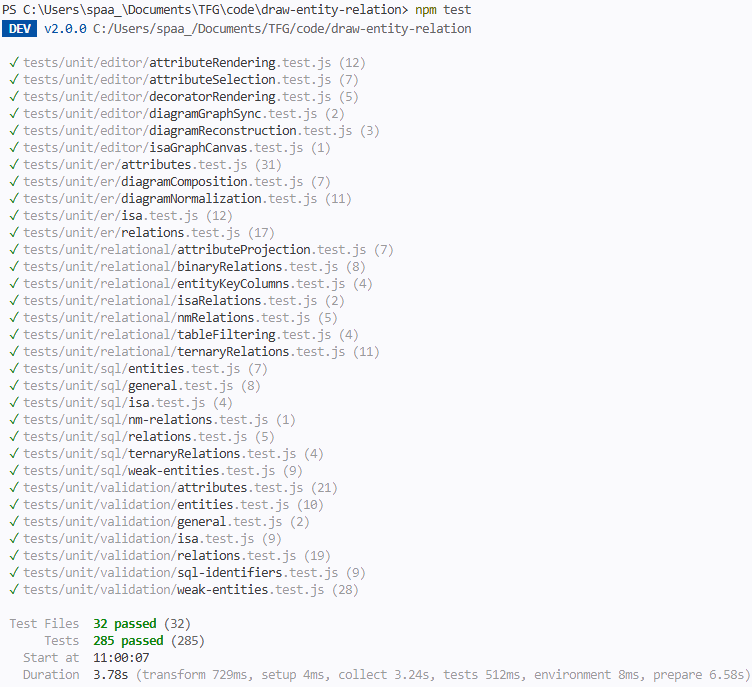
\includegraphics[width=0.92\textwidth,keepaspectratio]{img/tests_unitarios}
\caption{Ejecución de las pruebas unitarias del proyecto mediante Vitest.}
\label{fig:tests-unitarios}
\end{figure}


En la comprobación final realizada tras la limpieza y reorganización del código fuente, la batería de pruebas unitarias se ejecutó correctamente, con 32 ficheros de test y 285 pruebas superadas. Este resultado permite considerar que los cambios aplicados no rompieron las comprobaciones automáticas existentes.

No obstante, conviene interpretar estas pruebas con prudencia. Que una funcionalidad esté cubierta por pruebas unitarias no significa que todos sus casos de uso visuales estén completamente verificados, especialmente en las partes dependientes de mxGraph y de la interacción directa del usuario con el lienzo.

\subsection{Pruebas de extremo a extremo}

El proyecto también dispone de pruebas de extremo a extremo mediante Playwright. Estas pruebas permiten verificar flujos completos de uso desde el punto de vista del usuario, ejecutando la aplicación en un navegador controlado por la herramienta.

El comando definido para este tipo de pruebas es:

\begin{verbatim}
npm run test:e2e
\end{verbatim}

\begin{figure}[H]
\centering
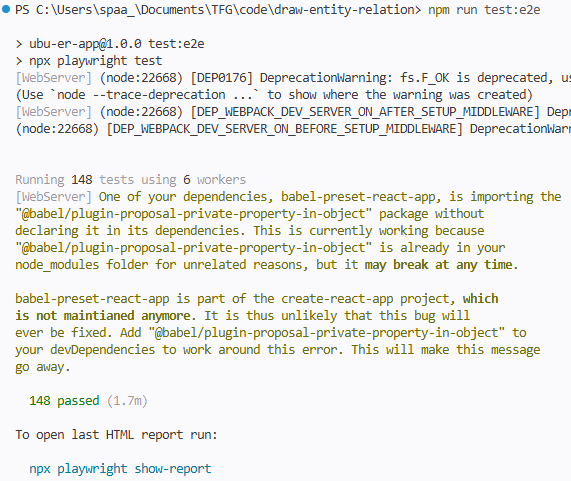
\includegraphics[width=0.92\textwidth,keepaspectratio]{img/tests_e2e}
\caption{Ejecución de las pruebas de extremo a extremo mediante Playwright.}
\label{fig:tests-e2e}
\end{figure}

Estas pruebas son especialmente útiles para comprobar escenarios en los que intervienen varios elementos de la aplicación: carga del editor, interacción con la interfaz, creación de elementos, validación de acciones y comportamiento general del sistema en navegador. En el contexto de este proyecto complementan a las pruebas unitarias, ya que permiten detectar regresiones en flujos completos que dependen de la interfaz y no solo de funciones aisladas.

En la ejecución mostrada se completaron correctamente 148 pruebas de extremo a extremo. Durante la ejecución pueden aparecer advertencias heredadas asociadas a \texttt{react-scripts} y a dependencias internas de Babel. Estas advertencias no impiden la ejecución de las pruebas ni suponen, por sí mismas, un fallo funcional de la aplicación.


\subsection{Cobertura de pruebas}

El proyecto incluye un script para obtener información de cobertura de las pruebas unitarias:

\begin{verbatim}
npm run test:coverage
\end{verbatim}

Este comando permite identificar qué partes del código están siendo ejercitadas por las pruebas automáticas. La cobertura debe utilizarse como una métrica de apoyo, no como único criterio de calidad. En una aplicación de estas características, una cobertura elevada puede no reflejar por completo la corrección de la interacción visual con el lienzo ni la usabilidad de los flujos de edición.

Por ello, la cobertura resulta útil para detectar zonas de lógica interna con poca validación automática, pero debe complementarse con revisión manual y pruebas de integración cuando se modifiquen comportamientos complejos.

\subsection{Construcción de producción}

La construcción de producción permite comprobar que la aplicación puede compilarse correctamente y generar los ficheros estáticos necesarios para su despliegue.

El comando utilizado es:

\begin{verbatim}
npm run build
\end{verbatim}

Este comando ejecuta previamente el script de generación de información de construcción y, después, lanza el proceso de \texttt{react-scripts build}. Si la compilación finaliza correctamente, se genera la carpeta \texttt{build/}, que contiene la versión optimizada de la aplicación.

Durante la comprobación final, la build se generó correctamente. Únicamente aparecieron advertencias heredadas asociadas a \texttt{react-scripts} y Babel, que no impidieron la generación de la aplicación ni bloquearon su ejecución.

\subsection{Revisión manual}

Además de las pruebas automáticas, se realizaron revisiones manuales del comportamiento de la aplicación en el navegador. Estas revisiones son importantes porque parte del sistema depende de la coordinación entre React, mxGraph, la representación interna del diagrama y la interacción directa del usuario.

Entre los aspectos revisados manualmente destacan:

\begin{itemize}
\item creación y edición de entidades, relaciones y atributos;
\item creación y configuración de jerarquías ISA;
\item selección simple y múltiple de elementos;
\item movimiento y borrado de varios elementos;
\item validación del diagrama;
\item transformación al modelo relacional;
\item generación de SQL compatible con PostgreSQL;
\item persistencia local;
\item importación y exportación JSON;
\item reconstrucción visual del diagrama importado;
\item exportación visual del lienzo;
\item ajuste de vista y uso del panel lateral.
\end{itemize}

Estas comprobaciones no sustituyen a las pruebas automáticas, pero permiten detectar regresiones visuales o de interacción que no siempre aparecen en pruebas unitarias. Un ejemplo de este tipo de revisión fue la detección de un problema de orden en el panel lateral, donde las secciones de selección y orden aparecían al final del panel en lugar de mostrarse junto a las herramientas principales.

\subsection{Comprobación recomendada antes de cerrar cambios}

Antes de considerar cerrado un cambio relevante en el código fuente, se recomienda ejecutar al menos la siguiente secuencia:

\begin{verbatim}
npm run lint
npm test -- --run
npm run build
\end{verbatim}

Si el cambio afecta a flujos completos de usuario, interacción visual, importación, exportación, persistencia o reconstrucción del lienzo, también se recomienda ejecutar:

\begin{verbatim}
npm run test:e2e
\end{verbatim}

y realizar una revisión manual en el navegador.

Esta pauta no garantiza por sí sola la ausencia completa de errores, pero reduce el riesgo de introducir regresiones en una aplicación heredada con acoplamiento entre modelo interno, representación visual y lógica de transformación.

La figura siguiente muestra una comprobación de análisis estático y construcción de producción. La ejecución de pruebas unitarias se documenta previamente en la Figura~\ref{fig:tests-unitarios}.

\begin{figure}[H]
\centering
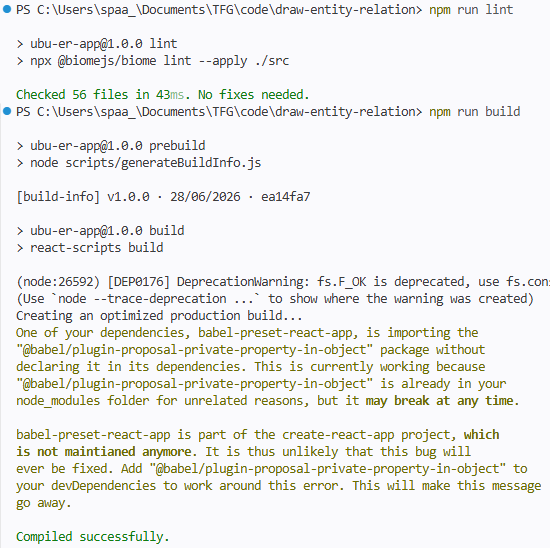
\includegraphics[width=0.92\textwidth,keepaspectratio]{img/comprobacion_final}
\caption{Comprobación de análisis estático y construcción de producción del proyecto.}
\label{fig:comprobacion-final}
\end{figure}
